\section{Part I: Pseudorandomness in Proof Complexty}

\begin{frame}
    \centering
    \usebeamerfont{title}\insertsectionhead

    \vspace{0.3cm}
    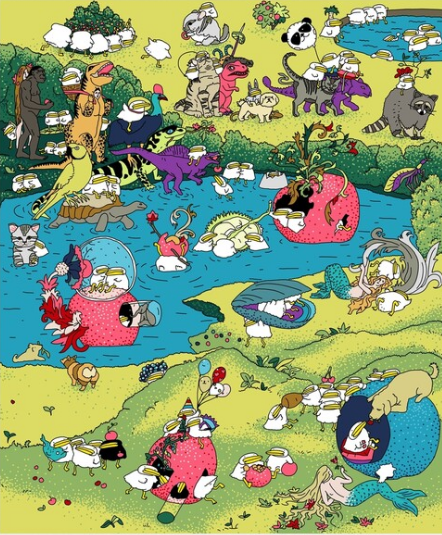
\includegraphics[scale = 0.3]{pics/utia-garden.png}
\end{frame}

\begin{frame}{Pseudorandom Generators}

    \begin{itemize}
        \item $G\colon \{0, 1\}^n \to \{0, 1\}^m$;
            \pause
        \item $\forall C \in \mathfrak{C}:$
            $$
                \abs{\Pr\limits_{x \in \{0, 1\}^n}[C(G(x)) = 1] -
                \Pr\limits_{y \in \{0, 1\}^m}[C(y) = 1]} \to 0;
            $$
            \pause
        \item $\textcolor{red}{\forall}b \stackrel{?}{\in} \Img(G)$;
            \pause
        \item Is the formula $\varphi_b \coloneqq "b \in \Img(G)"$ hard for a proof system?
    \end{itemize}

    \pause
    \vspace{0.3cm}
    Motivation:
    \begin{itemize}
        \item Pseudorandom generators against some algorithms;
        \item $\NP$ vs. $\Ppoly$;
        \item ``Unnatural proofs'';
        \item etc. 
    \end{itemize}
\end{frame}


\begin{frame}{Nisan--Wigderson Generators}

    \begin{minipage}{0.48\linewidth}
        \centering
        \begin{tikzpicture}

    \pgfmathsetseed{1000007}
    \foreach \i in {0, 1, ..., 5}{
        \node[graph-vert] (b\i) at
            (1.5, 0.4 * \i + 0.4) {};
    }

    \foreach \i in {0, 1, ..., 7}{
        \node[graph-vert = {LEIorange!80!black}{0.15cm}] (a\i) at
            (0, 0.4 * \i) {};

        \draw[->] (a\i) -- ++(-0.3, 0);

        \foreach \j in {0, 1, 2}{
            \pgfmathsetmacro{\temp}{random(0, 5)}
            \draw (a\i) -- (b\temp);
        }
    }

    \node[below = 0.2cm] at (a0) {$m$};
    \node[below = 0.2cm] at (b0) {$n$};
\end{tikzpicture}
    \end{minipage}
    \putpos{-40}{50}{
\includegraphics[scale = 0.1]{pics/utia-rest.png}}
    \begin{minipage}{0.48\linewidth}
        \begin{itemize}
            \item $\Delta$ is the left degree;
            \item $P(x_1, \dots, x_{\Delta})$ is a predicate.
        \end{itemize}
        
        \vspace{0.2cm}
        \pause
        \begin{itemize}
            \item Easy to compute;
            \item $m \le 2^{n^{\varepsilon}} \Rightarrow$ hard for $\AC_0$-circuits.
        \end{itemize}
    \end{minipage}

    \pause
    \vspace{0.3cm}
    \begin{minipage}{0.38\linewidth}
        \begin{itemize}
            \item Extended Frege \pause \alert{too strong}
                \pause
            \item Frege \pause \alert{too strong}
                \pause
            \item Resolution \pause \textcolor{blue}{nothing to do}
                \pause
            \item Something in between
        \end{itemize}
    \end{minipage}
    \pause
    \begin{minipage}{0.56\linewidth}
        \begin{lemma}
            Resolution with extension variables $\Leftrightarrow$ Extended Frege.
        \end{lemma}
    \end{minipage}
\end{frame}


\begin{frame}{Functional encoding [ABRW 00]}
    
    \pause
    \begin{minipage}{0.38\linewidth}
        \centering
        \begin{tikzpicture}

    \pgfmathsetseed{1000007}
    \foreach \i in {0, 1, ..., 5}{
        \node[graph-vert] (b\i) at
            (1.5, 0.4 * \i + 0.4) {};
    }

    \foreach \i in {0, 1, 3, 4, ..., 7}{
        \node[graph-vert = {LEIorange!80!black}{0.15cm}] (a\i) at
            (0, 0.4 * \i) {};

        \draw[->] (a\i) -- ++(-0.3, 0);

        \foreach \j in {0, 1, 2}{
            \pgfmathsetmacro{\temp}{random(0, 5)}
            \draw (a\i) -- (b\temp);
        }
    }

    \node[graph-vert, alt = <{3-5}>{fill = red!80}{fill = LEIorange!80!black}] (a2) at (0, 0.8) {};
    \draw[->] (a2) -- ++(-0.3, 0);
    \foreach \j in {0, 1, 2}{
        \pgfmathsetmacro{\temp}{random(0, 5)}
        \draw[alt = <{3-5}>{red, thick}{}] (a2) -- (b\temp);
    }

    \node[below = 0.2cm] at (a0) {$m$};
    \node[below = 0.2cm] at (b0) {$n$};
\end{tikzpicture}
    \end{minipage}
    \begin{minipage}{0.58\linewidth}
        Fix some $b \notin \Img(G)$. For all $i \in [m]$:
        \begin{itemize}
            \item $\mathrm{N}(i) \coloneqq \{x_1, x_2, \dots, x_{\Delta}\}$;
                \pause
            \item encode $b_i = P(x_1, x_2, \dots, x_{\Delta})$ in CNF;
                \pause
            \item for all $f(x_1, x_2, \dots, x_{\Delta})$:
                \begin{itemize}
                    \item $y_f$ is a variable;
                    \item $y_f = 1 \Leftrightarrow f(x_1, x_2, \dots, x_{\Delta}) = 1$;
                \end{itemize}
                \pause
            \item $(y_{g_1}^{c_1} \lor y_{g_2}^{c_2} \lor y_{g_3}^{c_3} \cdots \lor
                y_{g_\ell}^{c_{\ell}})$ iff:
                $$
                    P(x) = b_i \models g_j(x) = c_j;
                $$
            \item  \pause $f \coloneqq g \oplus h \Leftrightarrow
                \begin{cases}
                    y_g \lor \neg y_h \lor y_f \\
                    \neg y_g \lor y_h \lor y_f \\
                    y_g \lor y_h \lor \neg y_f \\
                    \neg y_g \lor \neg y_h \lor \neg y_f.
                \end{cases}$
        \end{itemize}
    \end{minipage}

    \pause
    \vspace{0.2cm}
    \begin{minipage}[t][3cm][t]{0.32\linewidth}
        \centering
        $\mathbf{m \ll n^2}$

        \pause
        \vspace{0.2cm}
        $\exp\left[\frac{n^2}{m \alert<14->{2^{2^{\Delta}}}} \right]$

        \vspace{0.2cm}
        [ABRW 00]
    \end{minipage}
    \pause
    \begin{minipage}[t][3cm][t]{0.32\linewidth}
        \centering
        $\mathbf{m \ll n^{\log n}}$

        \pause
        \vspace{0.2cm}
        $n^{\omega(1)}$

        \vspace{0.2cm}
        [Razb 14]

        \pause
        \vspace{0.1cm}
        \alert{weaker encoding}
    \end{minipage}
    \pause
    \begin{minipage}[t][3cm][t]{0.32\linewidth}
        \centering
        $\mathbf{m \gg n^{\log n}}$

        \pause
        \vspace{0.2cm}
        
\includegraphics[scale = 0.05]{pics/utia-cry.png}

        \pause
        \vspace{0.1cm}
        \alert{not for NW generator}
    \end{minipage}
\end{frame}


\begin{frame}{Results}

    \begin{theorem}
        \begin{itemize}
            \item $G$ is a $(r, \Delta, (1 - \varepsilon) \Delta)$-expander;
            \item $P$ is a \textcolor{blue}{good} predicate
        \end{itemize}
        $\Rightarrow$ any resolution proof of $\langcplx{PRG}_{G, P, b}$ has size
        $\exp\left[\Omega\left( \frac{\varepsilon^5 r^2}{\alert{2^{6 \varepsilon \Delta}} m} \right) \right]$.
    \end{theorem}

    \pause

    \begin{minipage}{0.4\linewidth}
        \begin{itemize}
            \item $m \coloneqq n^{2 - \delta}$;
            \item $\Delta \coloneqq \log^{2 - \delta} n$;
            \item $G$ is a random graph.
        \end{itemize}
    \end{minipage}
    \begin{minipage}{0.1\linewidth}
        $\Rightarrow$
    \end{minipage}
    \begin{minipage}{0.4\linewidth}
        Resolution size: $\exp[n^{\delta}]$.
    \end{minipage}

    \pause
    \vspace{0.4cm}
    \begin{minipage}[t][1cm][t]{0.48\linewidth}
        \centering
        $\mathbf{\Delta \ll \log\log n}$
        
        \pause
        \vspace{0.2cm}
        Resolution proof $\approx$ resolution proof without extension vars [ABRW 00]
    \end{minipage}
    \pause
    \begin{minipage}[t][3cm][t]{0.48\linewidth}
        \centering
        $\mathbf{\Delta \gg \log \log n}$

        \pause
        \vspace{0.2cm}
        
\includegraphics[scale = 0.05]{pics/utia-hz.png}
    \end{minipage}
\end{frame}